\section{Area-by-Area}
\label{sec:area-by-area}

In this section, each of the semantic areas introduced in Section \ref{subsec:semantic-areas} will be explored in depth and, in particular, the main elements that comprise it will be described. Bold font will be used to indicate classes, monospaced font for \acp{URI}, and italic font for properties. The prefixes in Table \ref{tab:ontopia-ontologies} will be used for \acp{URI}.

\subsection{Demographic Observations and Events}
\label{subsec:demographic-observations}

This semantic area is represented in Figure \ref{fig:demographic-sa}, and comprehends the classes and the properties that describe demographic observations and events for the domains of demographic statistics, civil status, tourism, events, schools, and organizations.

\begin{sidewaysfigure}[!ht]
  \centering
  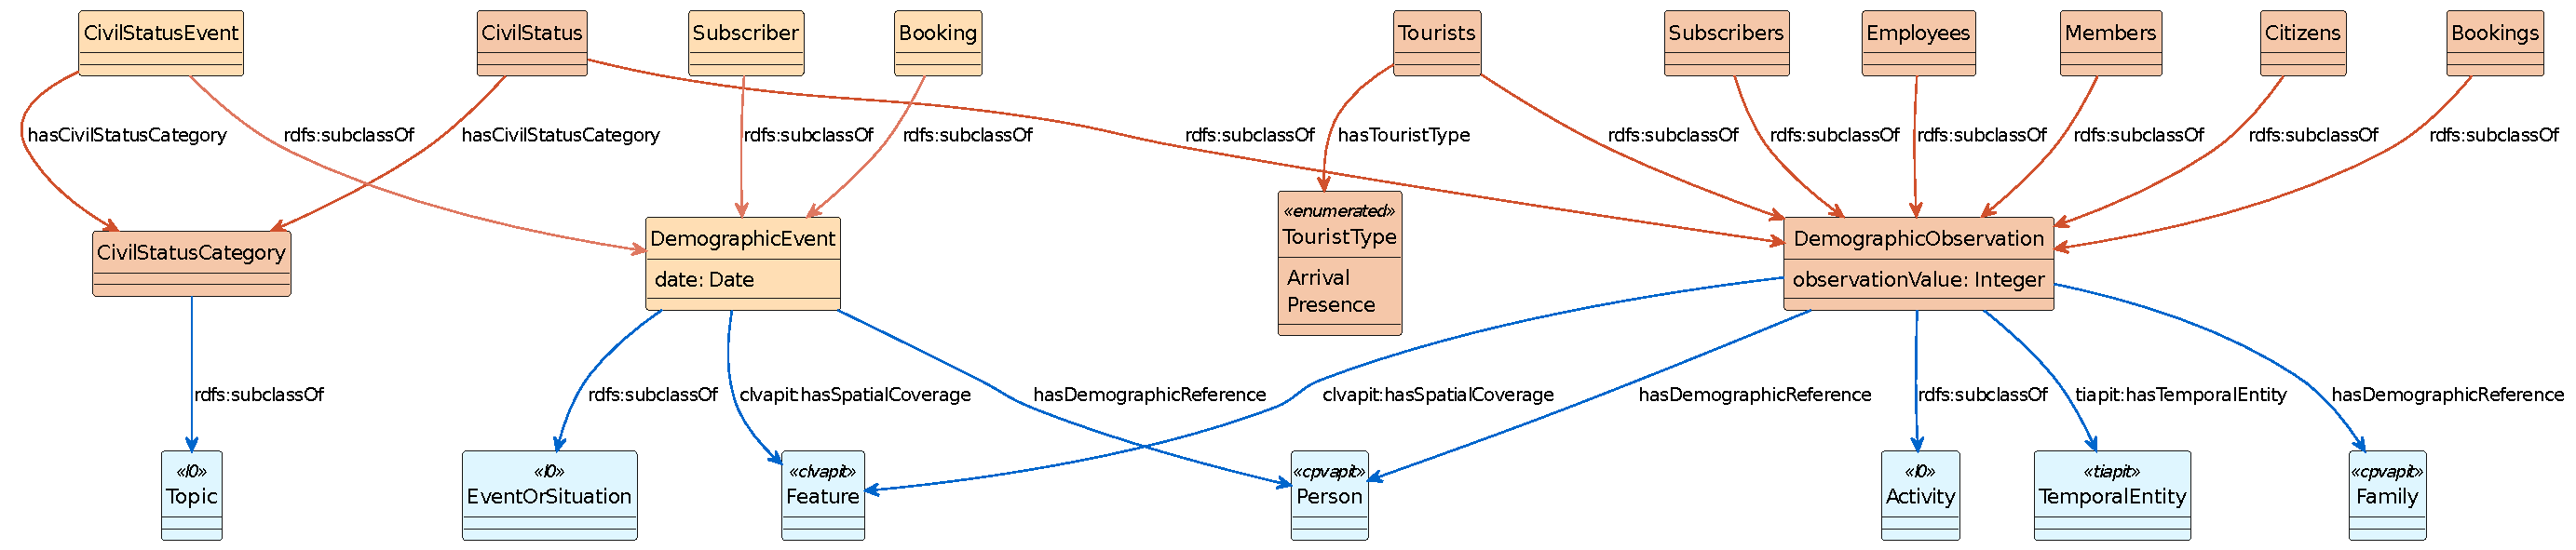
\includegraphics[width=\columnwidth]{images/ontoim/demographic}
  \caption{Demographic Observations and Events semantic area.}
  \label{fig:demographic-sa}
\end{sidewaysfigure}

There are two main classes in this area. The \textbf{Demographic Observation} class (\verb#:DemographicObservation#), and the \textbf{Demographic Event} (\verb#:DemographicEvent#) class. This makes it possible to represent data either in aggregate form (e.g., the number of marriages in a year) or, where possible, as individual events (e.g., a wedding occurred on a particular day).

The class \textbf{Demographic Observation}, which is a subclass of the \textbf{Activity} class (\verb#l0:Activity#) has the data property \textit{observationValue} (\verb#xsd:nonNegativeInteger#), which represents the quantity of the observation (e.g. the number of citizens). Through the properties \textit{hasTemporalEntity} and \textit{hasSpatialCoverage}, \textbf{DemographicObservation} is connected to \textbf{TemporalEntity} (\verb#tiapit:TemporalEntity#) and \textbf{Feature} (\verb#clvapit:Feature#) respectively. In this way it is possible to define the time and space to which the observation refers. To get more accurate statistics, it may be useful to distinguish observations by gender, citizenship or other characteristics. Instead of adding different properties for each of these characteristics, you can use the \textit{hasDemographicReference} property, which connects \textbf{DemographicObservation} to a \textbf{Person} (\verb#cpvapit:Person#) class or \textbf{Family} (\verb#cpvapit:Family#) class for observations about families. These classes then reference the observed characteristics.

Different type of observations are modeled using subclasses of the class \textbf{DemographicObservation}. The main subclasses are:

\begin{description}
  \item[Tourists]  (\verb#:Tourists#) To describe observations about the number of tourists. We can distinguish two type of observations about tourism: arrivals and presences. The \textit{hasTouristType} property connect \textbf{Tourists} to the enumerated class \textbf{TouristType} (\verb#TouristiType#), which can be \verb#:Arrival# or \verb#Presence#;
  \item[CivilStatus]  (\verb#:CivilStatus#) To describe the number of civil status events (e.g. births, deaths, marriages, \etc). The typology of the event is defined through the class \textbf{CivilStatusCategory} (\verb#:CivilStatusCategory#), connected by the property \textit{hasCivilStatusCategory}. The available categories are defined in a controlled vocabulary following the entries in the ISTAT D.7.A model\footnote{\url{https://purl.archive.org/istat-d7a-sona-2021}} of civil status statistics.
  \item[Subscribers] (\verb#:Subscribers#) This subclass is used to describe observations about subscribers to events, school, and courses.
\end{description}

The remaining subclasses, which doesn't have additional properties, are: \textbf{Employees} (\verb#:Employees#), \textbf{Members} (\verb#:Members#), \textbf{Citizens} (\verb#:Citizens#), and \textbf{Bookings} (\verb#:Bookings#). They describe respectively: (1) the number of employees that works in a organization; (2) the number of members of an association; (3) demographic observation on the population; (4) the number of bookings in a accommodation facility.

\paragraph*{}
The \textbf{DemographicEvent} class is similar to \textbf{DemographicObservation}, but, as said before, is used to represent singular events. It shares with the latter the \textit{hasDemographicReference} and \textit{hasSpatialCoverage} properties, but it has the property \textit{date}, which defines the date on which the event occurred. Different subclasses are used to model specific types of events. In particular, such subclasses are: (1) \textbf{CivilStatusEvent} (\verb#:CivilStatusEvent#), which is the equivalent of \textbf{CivilStats} for the observations; (2) \textbf{Subscriber} (\verb#:Subscriber#), to model a single registration to an event, school or course; (3) \textbf{Booking} (\verb#:Booking#), to describe a single reservation to an accommodation facility.

\subsection{Facilities and Cadastral Data}
\label{subsec:facilities}

Figure \ref{fig:facilities-sa} represent the semantic area of facilities and cadastral data, which are used to describe schools, hospitals, green zones \etc.

\begin{figure}[!ht]
  \centering
  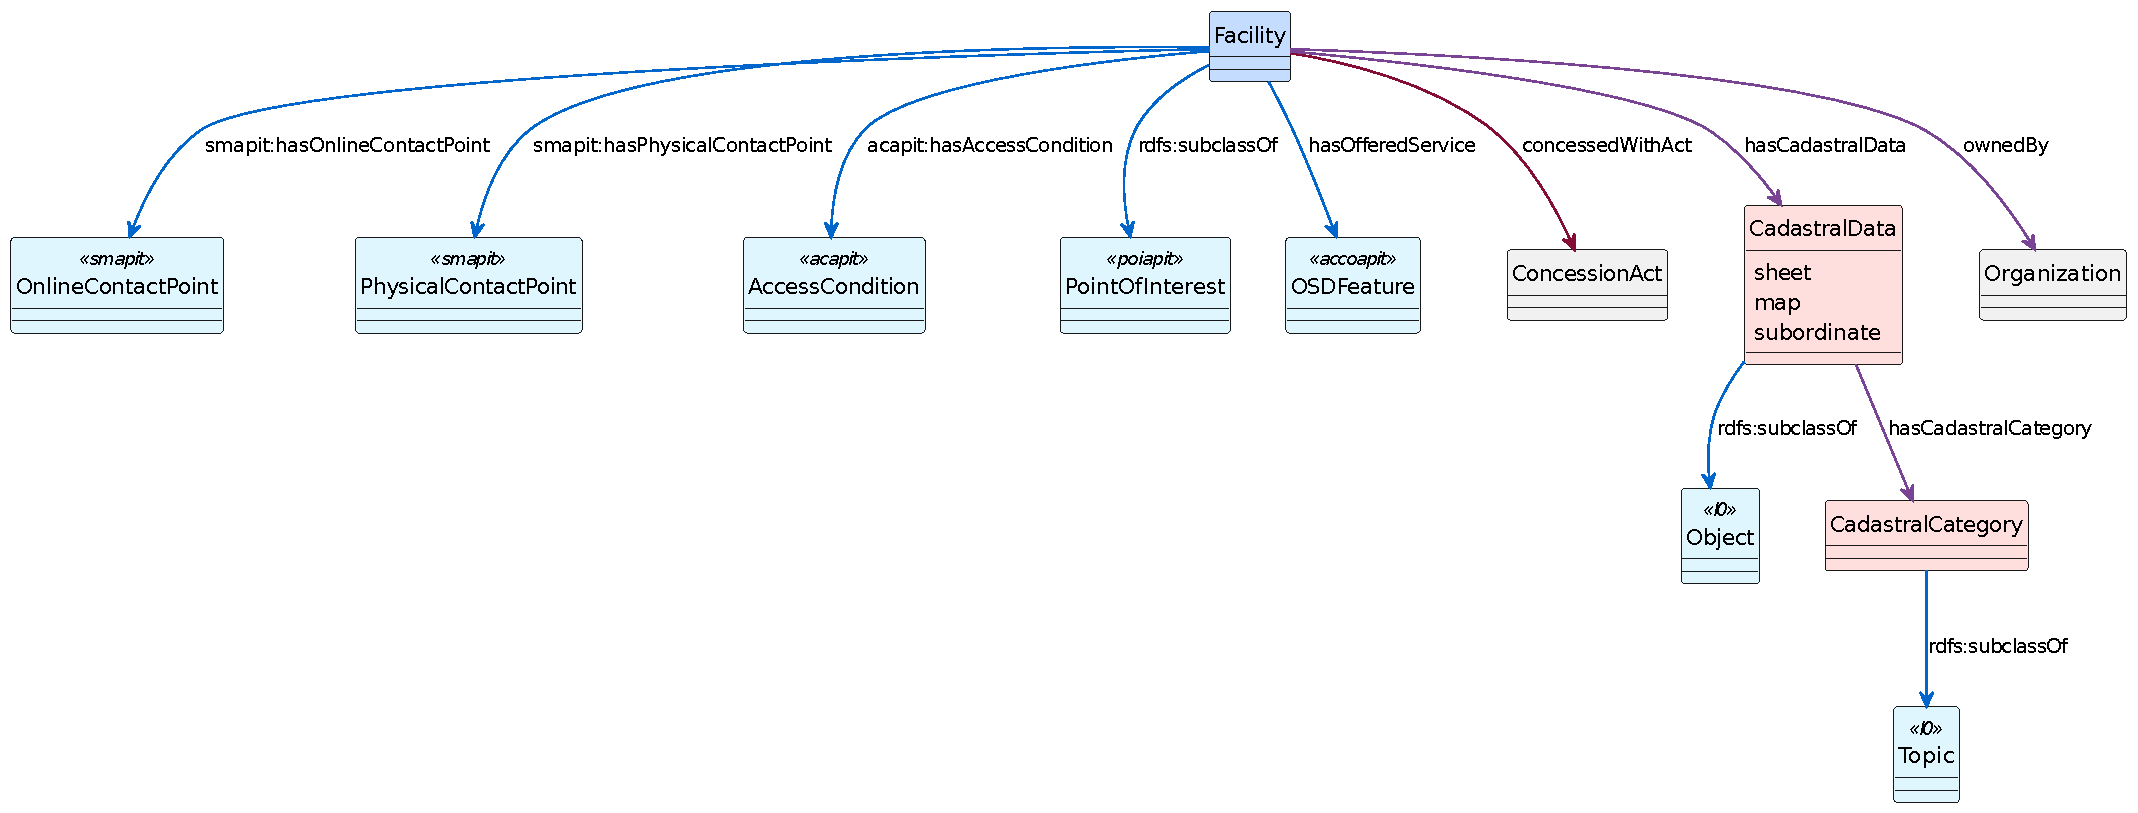
\includegraphics[width=\columnwidth]{images/ontoim/facilities}
  \caption{Facilities and Cadastral Data semantic area.}
  \label{fig:facilities-sa}
\end{figure}

The main class is \textbf{Facility} (\verb#:Facility#), which is a subclass of the \verb#POI_AP-IT#'s \textbf{PointOfInterest} class (\verb#poiapit:PointOfInterest#), and from which it inherits all the properties. The properties \textit{hasOnlineContactPoint}, \textit{hasPhysicalContactPoint}, and \textit{hasAccessConditions} connect the \textbf{Facility} class respectively to: (1) \textbf{OnlineContactPoint} (\verb#smapit:OnlineContactPoint#), which defines online contact points such as emails, social network usernames, websites, and telephones; (2) \textbf{PhysicalContactPoint} (\verb#smapit:PhysicalContactPoint#), which describes the address or the Point of Interest where the facility is located; (3) \textbf{AccessCondition} (\verb#acapit:AccessCondition#), which defines the facility opening hours. The \textbf{OSDFeature} class (\verb#accoapit:OSDFeature#) is connected through the property \textit{hasOfferedService}, and it is used to describe services and features that the facility offers (e.g. air conditioning, food service, parking, \etc).

A facility can be granted for use to an organization or person through a deed of grant. This situation is described by the property \textit{concessedWithAct} and the class \textbf{ConcessionAct} (\verb#:ConcessionAct#), which is described in Section \ref{subsec:transparency}.

\paragraph*{}
Finally, a facility is identified in the land registry by one or more cadastral data. The class \textbf{CadastralData} (\verb#:CadastralData#) stores this information, and it is connected to the \textbf{Facility} class through the \textit{hasCadastralData} property. A facility has also a cadastral category, defined by the class \textbf{CadastralCategory} (\verb#:CadastralCategory#). The elements of this class must be defined according to a controlled vocabulary that store the available cadastral categories.\footnote{\url{https://purl.archive.org/age-categorie-catastali}}

\subsection{Organizations and Associations}
\label{subsec:organizations-associations}

This semantic area is represented in Figure \ref{fig:organizations-sa}, and covers the domains of public and private organizations, and associations. The area was designed following the structure of the data provided by the Camera di Commercio.\footnote{\url{https://www.mn.camcom.gov.it/files/RegistroImprese/Legenda-elenchi.pdf}}

\begin{figure}[!ht]
  \centering
  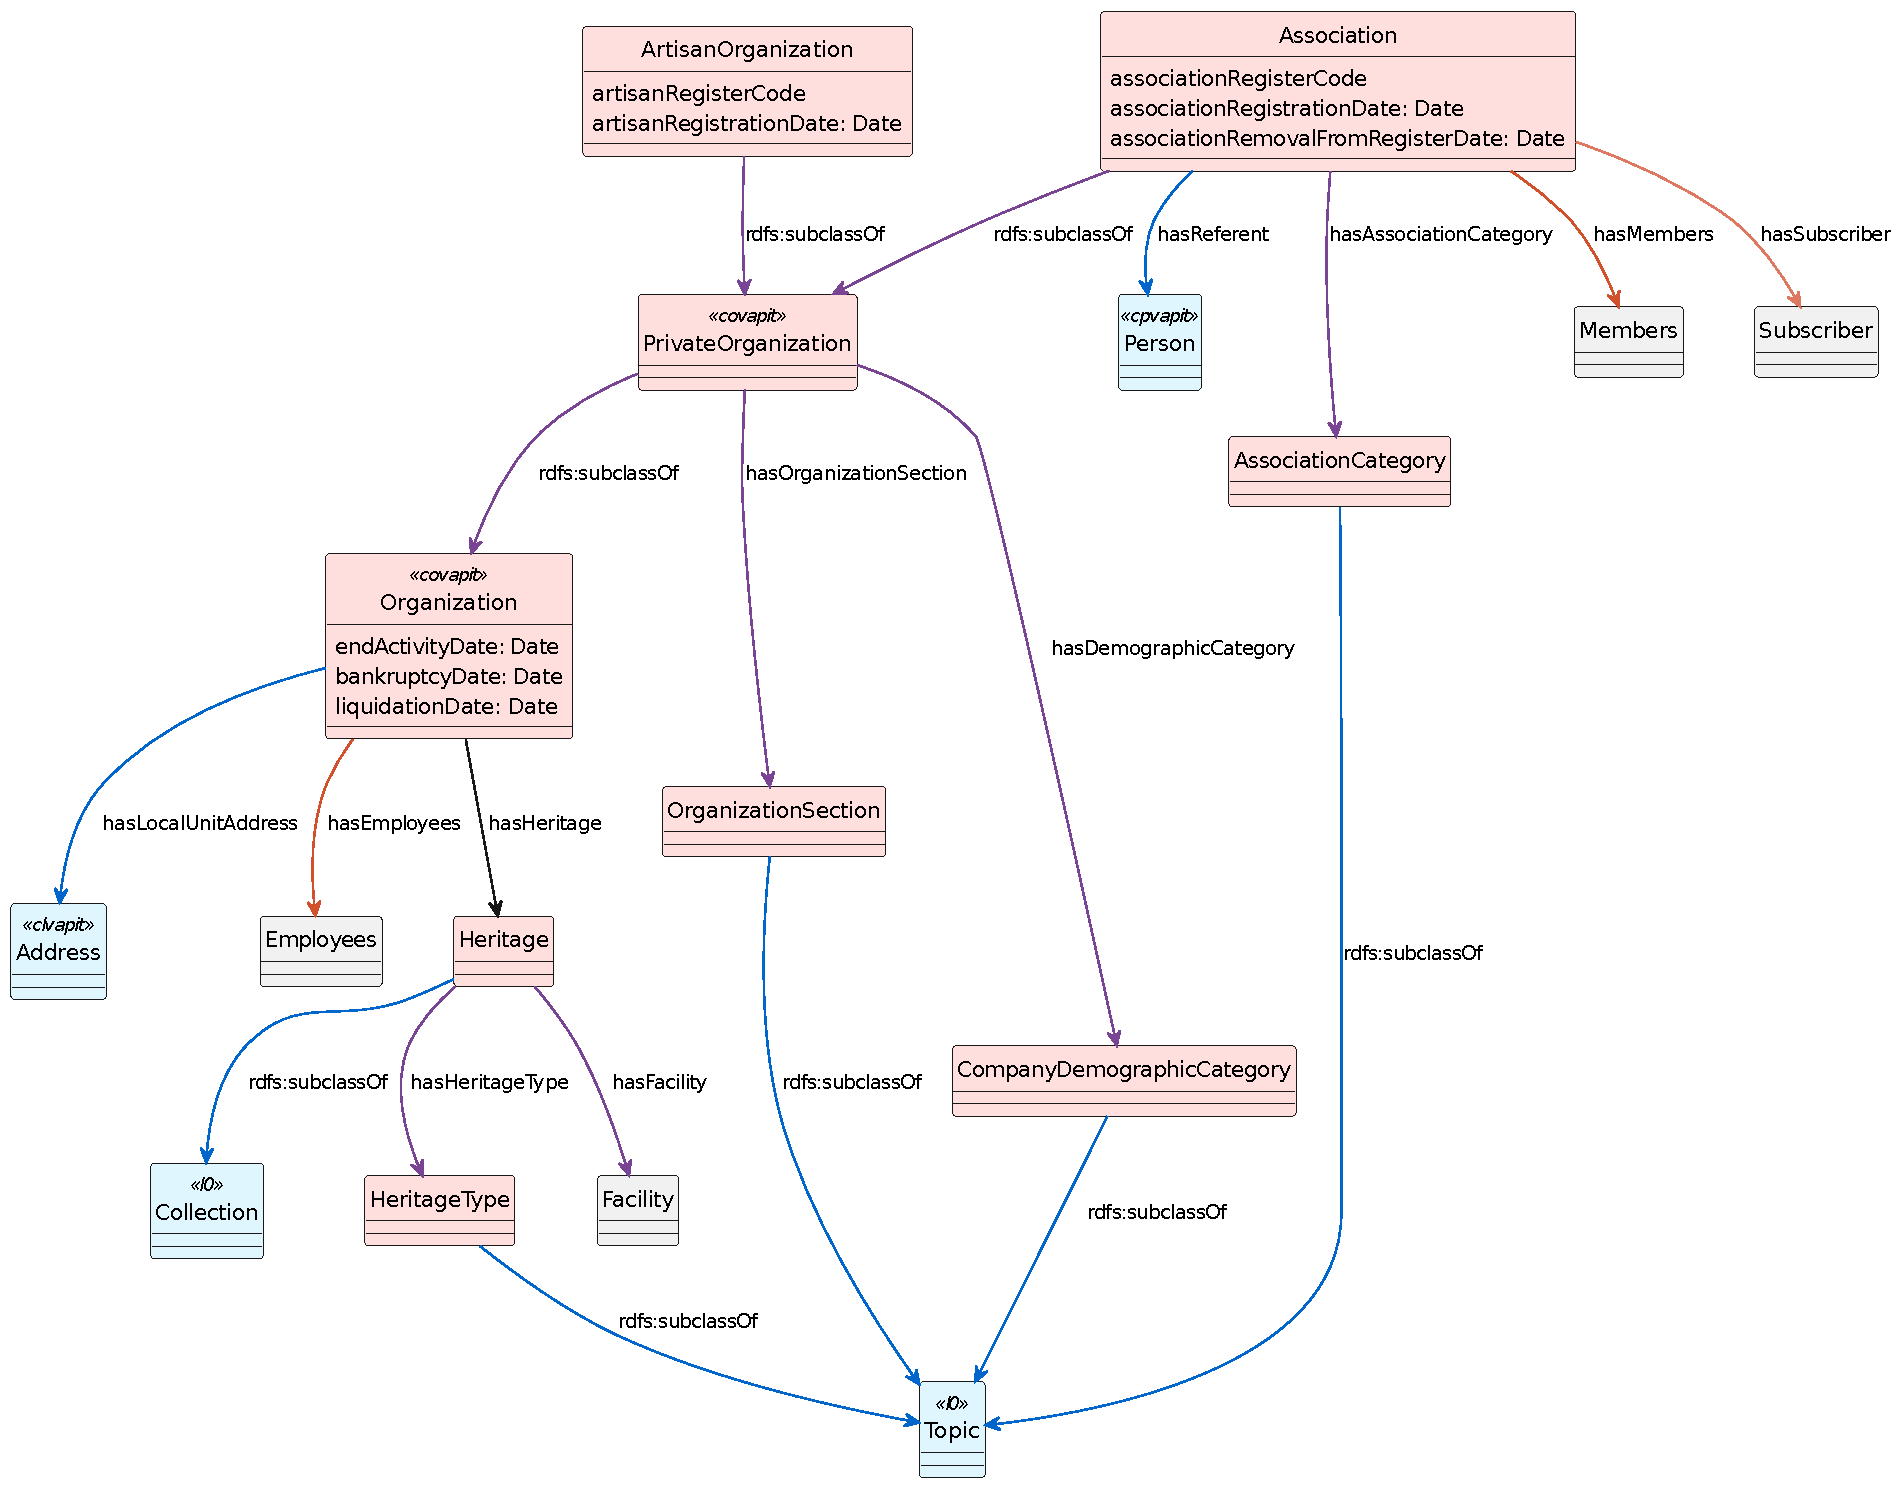
\includegraphics[width=\columnwidth]{images/ontoim/organizations}
  \caption{Organizations and Associations semantic area.}
  \label{fig:organizations-sa}
\end{figure}

Three data properties concerning events in the life cycle of an organization have been added to the \verb#COV_AP-IT#'s \textbf{Organization} class (\verb#covapit:Organization#). These properties, of type \verb#xsd:date#, are \textit{endActivityDate}, \textit{bankruptcyDate}, and \textit{liquidationDate}.

The property \textit{hasLocalUnitAddress} connects the \textbf{Organization} class to an \textbf{Address} class (\verb#clvapit:Address#), and it is used to store the addresses of one or more local units of the organization. It should also be specified that an organization may have its primary address in another city and a local unit in the municipality concerned. In that case, the Camera di Commercio provides only the address of the latter, specifying that it is a local unit.

For what concern demographic observations, as specified in Section \ref{subsec:demographic-observations}, the \textbf{Employees} class describes the number of employees that works in the organization.

This semantic area also extends the \verb#COV_AP-IT#'s \textbf{PrivateOrganization} class (\verb#covapit:PrivateOrganization#), which is a subclass of an \textbf{Organization}. The property \textit{hasOrganizationSection} connect the company to the \textbf{OrganizationSection} class (\verb#:OrganizationSection#). The elements of this class are defined in a controlled vocabulary created from the sections provided by the Camera di Commercio. Another controlled vocabulary defines the elements that must be used for the \textbf{CompanyDemographicCategory} class (:CompanyDemographicCategory), which defines whether the enterprise is a youth, female or foreign enterprise.

\subsection{Transparency}
\label{subsec:transparency}

\begin{figure}[!ht]
  \centering
  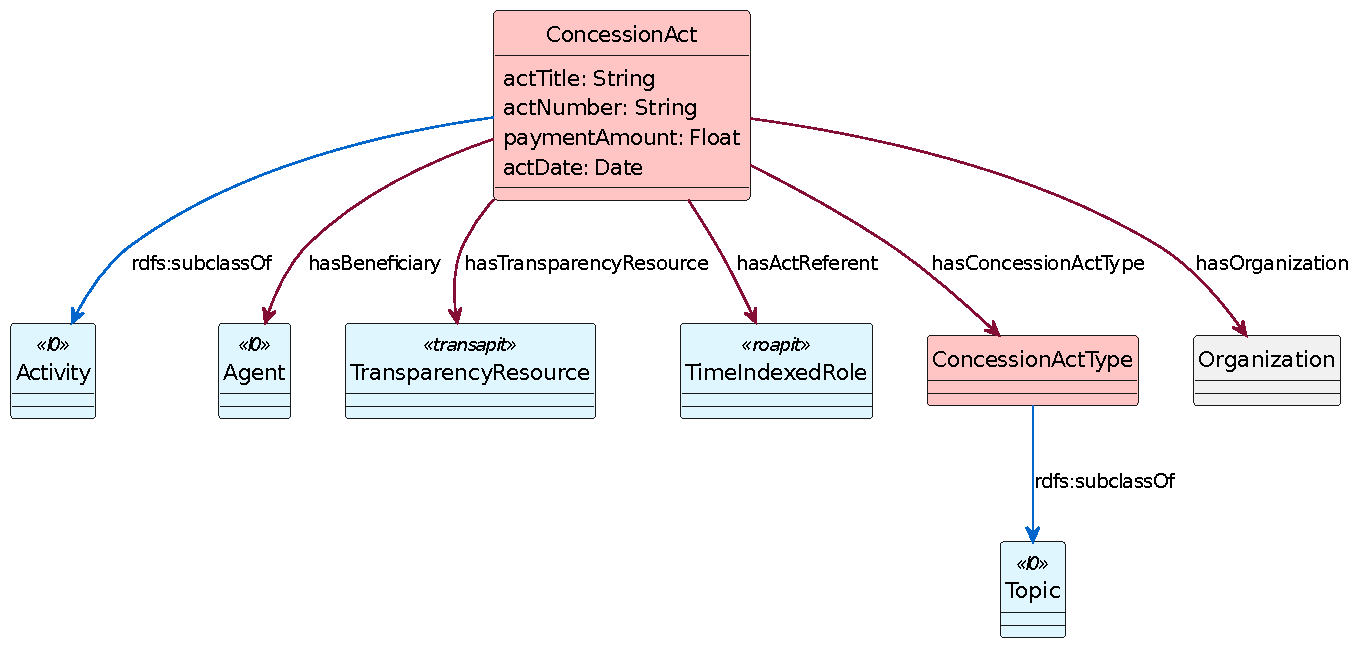
\includegraphics[width=\columnwidth]{images/ontoim/transparency}
  \caption{Transparency semantic area.}
  \label{fig:transparency-sa}
\end{figure}

\subsection{Roads and Traffic}
\label{subsec:roads-traffic}

\begin{sidewaysfigure}[!ht]
  \centering
  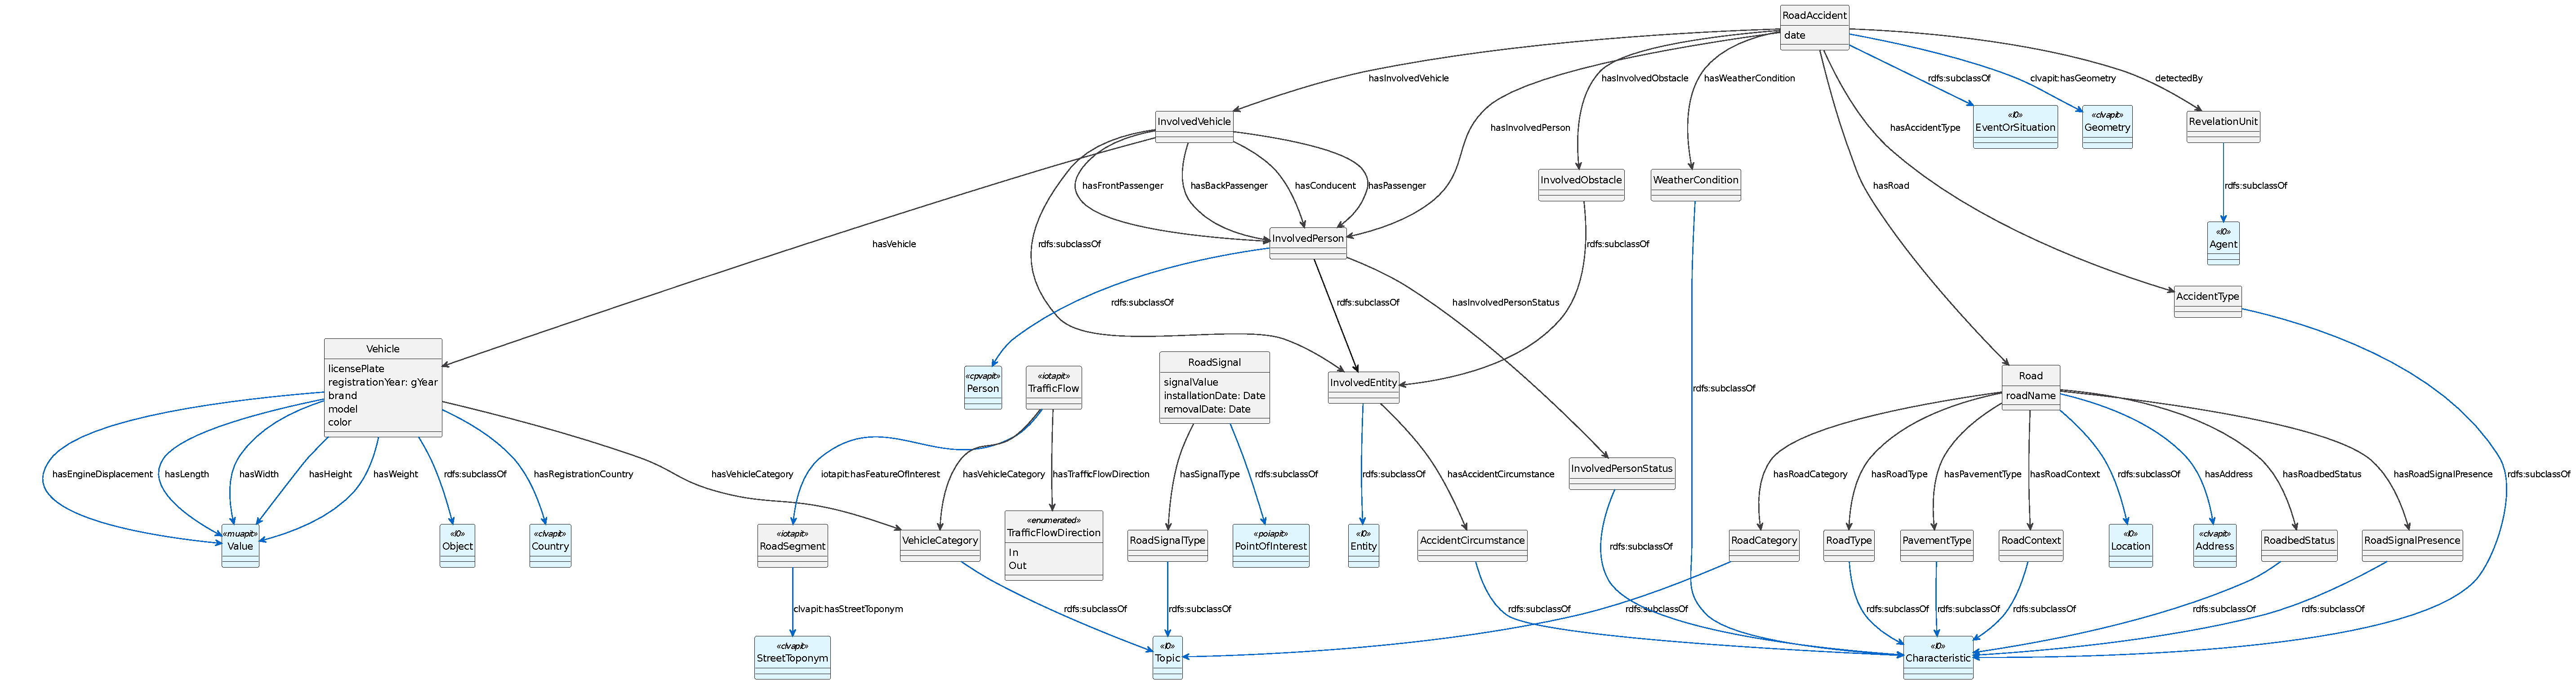
\includegraphics[width=\columnwidth]{images/ontoim/roads}
  \caption{Roads and Traffic semantic area.}
  \label{fig:roads-sa}
\end{sidewaysfigure}

\subsection{Schools}
\label{subsec:schools}

\begin{sidewaysfigure}[!ht]
  \centering
  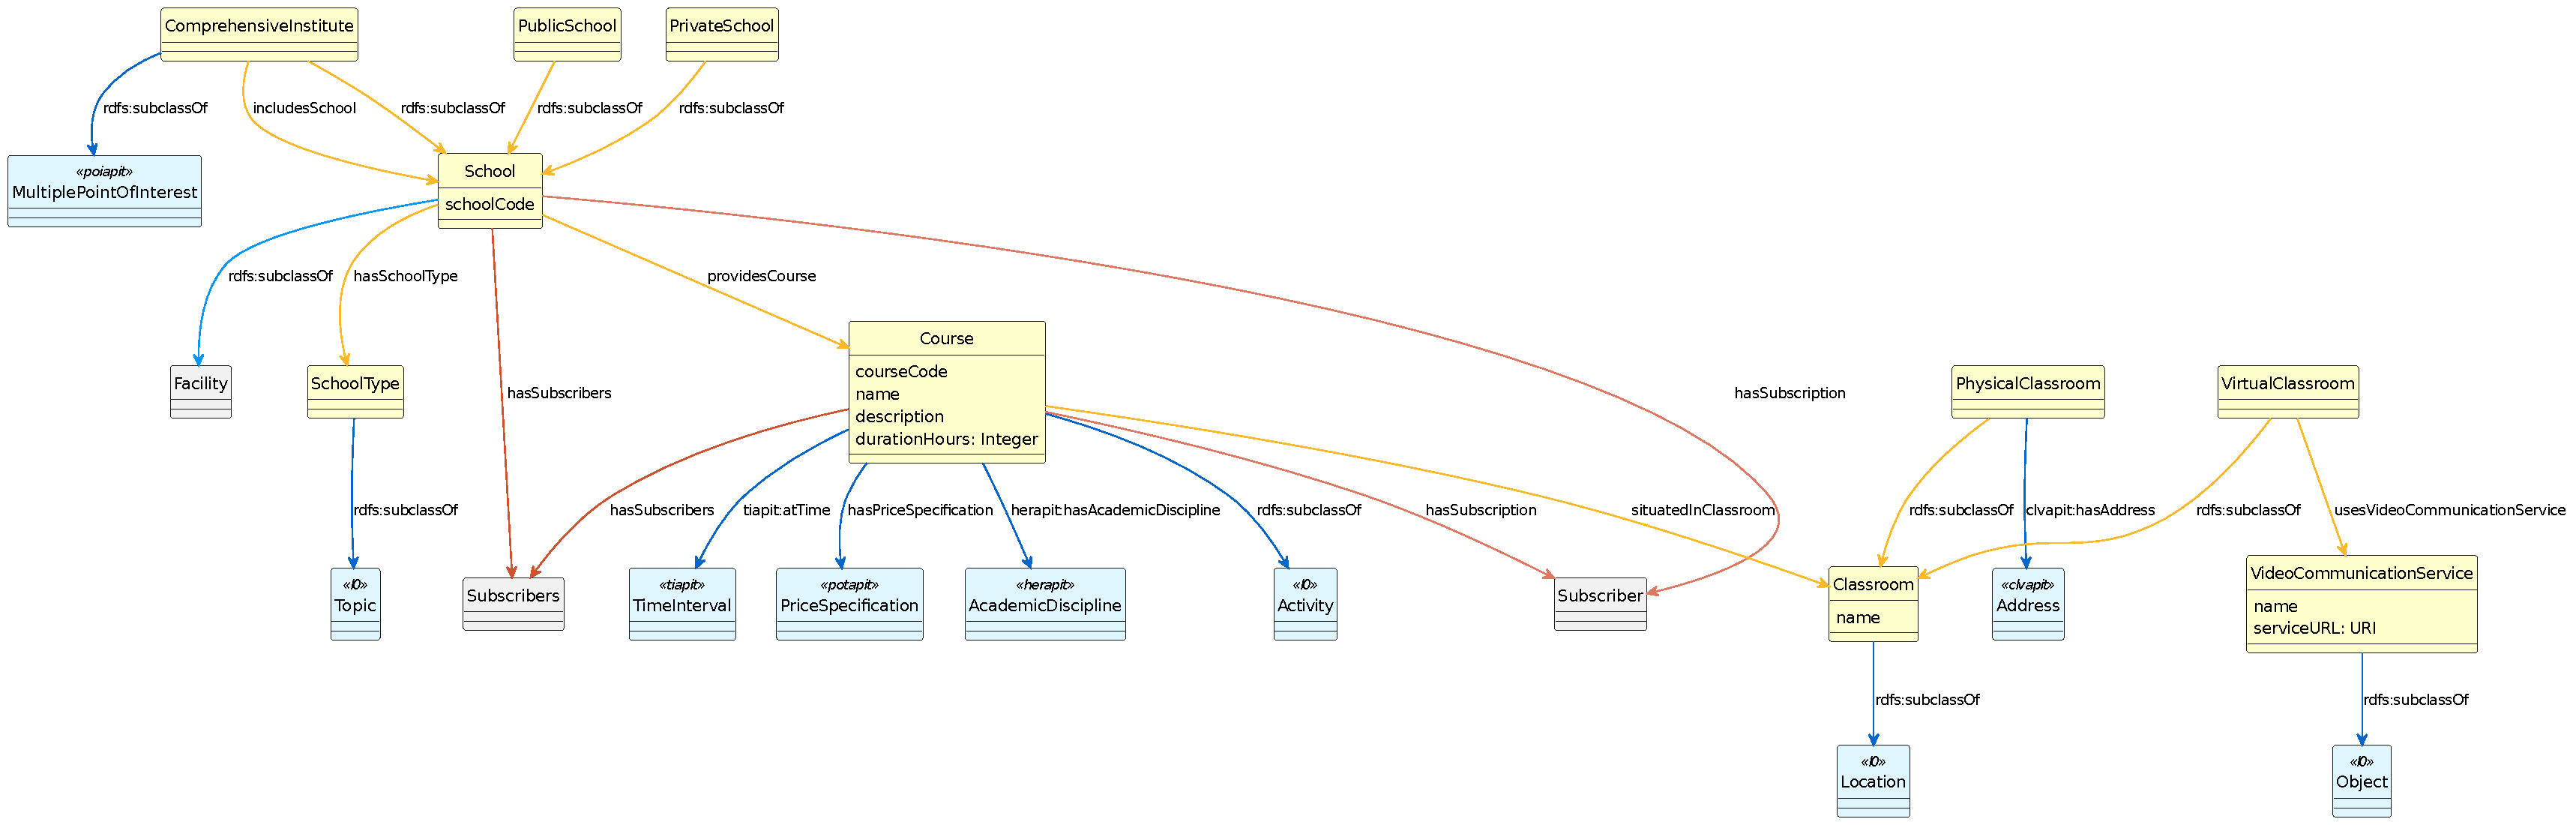
\includegraphics[width=\columnwidth]{images/ontoim/schools}
  \caption{Schools semantic area.}
  \label{fig:schools-sa}
\end{sidewaysfigure}

\subsection{Green Zones and Plants}
\label{subsec:green-zones}

\begin{figure}[!ht]
  \centering
  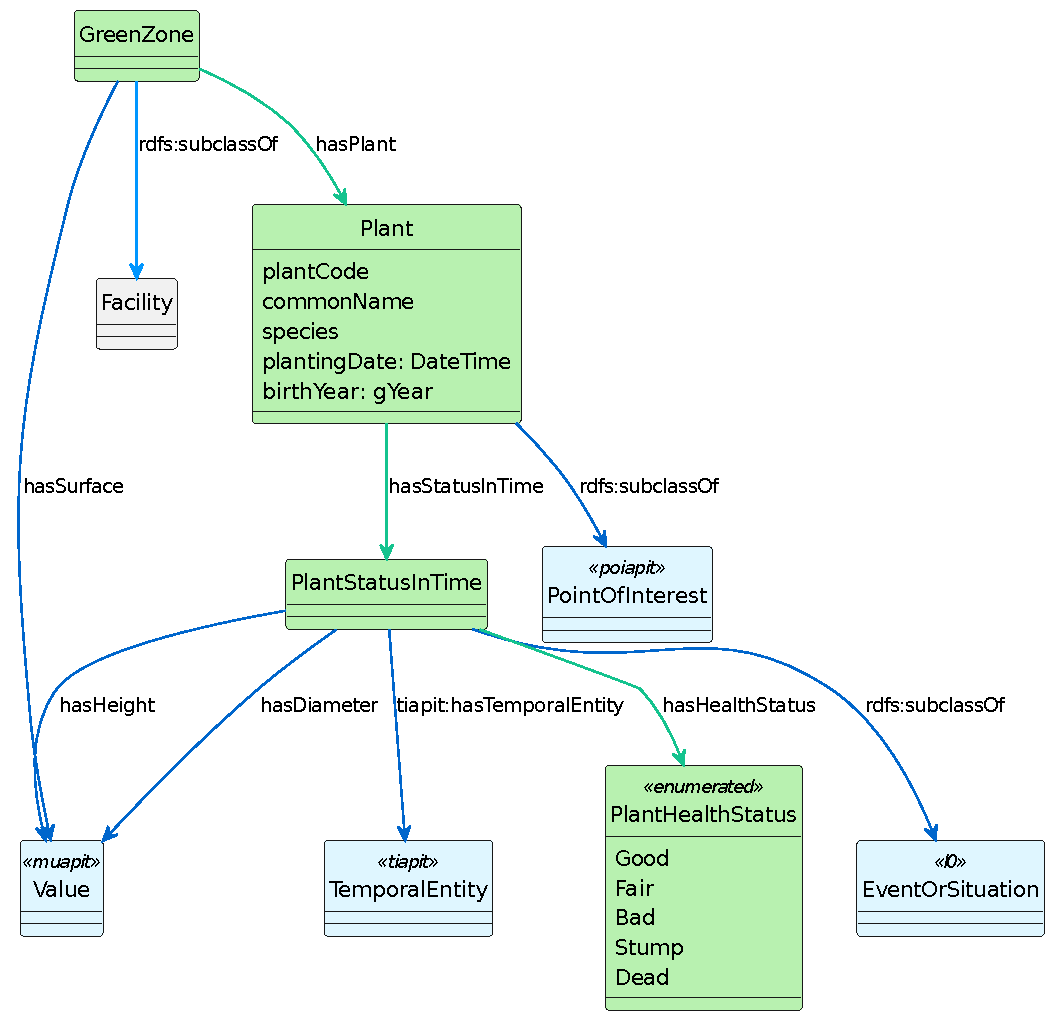
\includegraphics[width=0.6\columnwidth]{images/ontoim/green}
  \caption{Green Zones and Plants semantic area.}
  \label{fig:green-sa}
\end{figure}

\subsection{Hospitals}
\label{subsec:hospitals}

\begin{figure}[!ht]
  \centering
  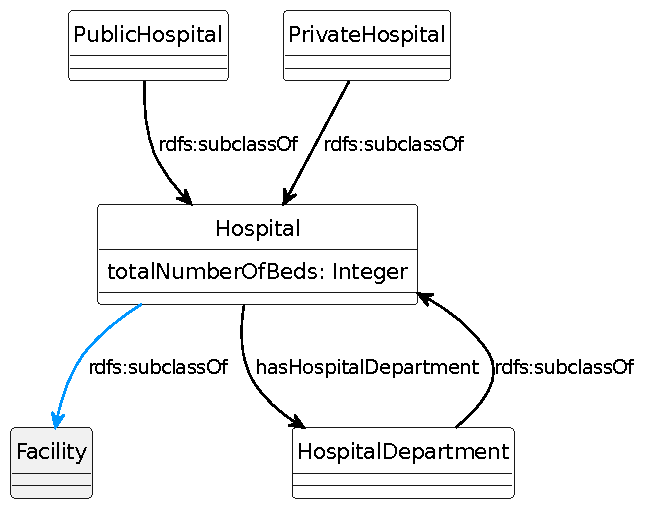
\includegraphics[width=0.5\columnwidth]{images/ontoim/hospitals}
  \caption{Hospitals semantic area.}
  \label{fig:hospitals-sa}
\end{figure}

\subsection{Waste Production}
\label{subsec:waste-production}

\begin{figure}[!ht]
  \centering
  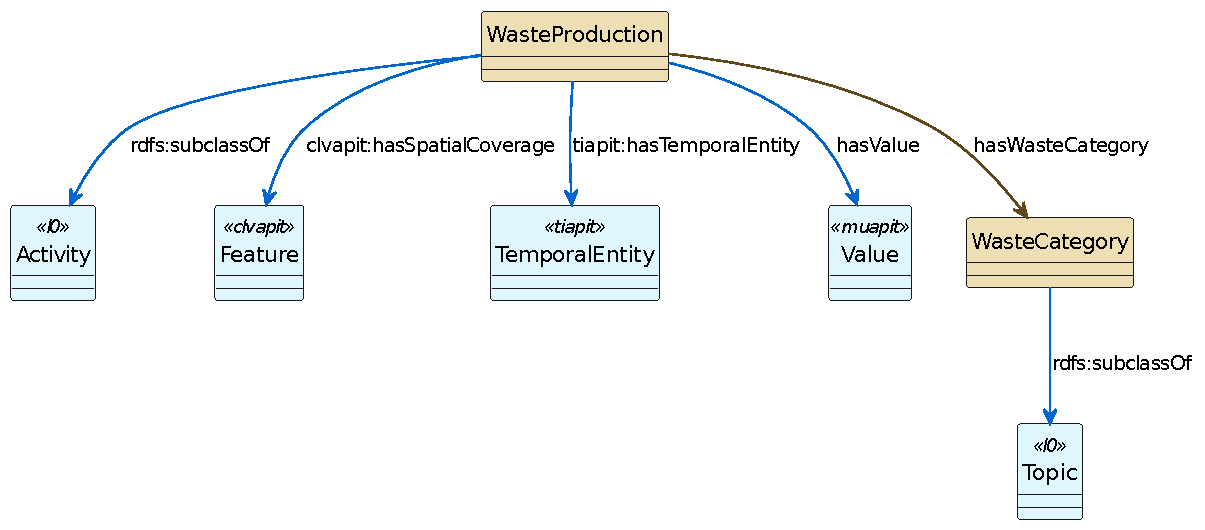
\includegraphics[width=\columnwidth]{images/ontoim/waste}
  \caption{Waste Production semantic area.}
  \label{fig:waste-sa}
\end{figure}